\documentclass[a4paper, 11pt]{book}
\usepackage{/home/nicolas/Documents/Enseignement/Prepa/bpep/fichiers_utiles/preambule}

\newcommand{\dsNB}{16}
\makeatletter
\renewcommand{\@chapapp}{Kh\^olles MPSI3 -- semaine \dsNB}
\makeatother

% \toggletrue{corrige}  % décommenter pour passer en mode corrigé

% IMPORTS automatiques
\newcommand{\f}[2]{{
		\mathchoice
		{\dfrac{#1}{#2}}
		{\dfrac{#1}{#2}}
		{\frac{#1}{#2}}
		{\frac{#1}{#2}}
}}

\newcommand{\e}[1]{{}_{\text{#1}}}
\renewcommand{\a}[0]{\alpha}
\newcommand{\w}[0]{\omega}

\usepackage{physics}

 % fin des IMPORTS automatiques

\begin{document}

\chapter{Sujet 1\siCorrige{\!\!-- corrig\'e}}
\section{Question de cours}

Retrouver l'équation différentielle sur $\tt$ du pendule simple non amorti à
l'aide du TPM.

\resetQ
\subimport{/home/nicolas/Documents/Enseignement/Prepa/bpep/exercices/TD/ski/}{sujet.tex}

\chapter{Sujet 2\siCorrige{\!\!-- corrig\'e}}
\section{Question de cours}

Énoncer et démontrer les théorèmes de la puissance mécanique et de l'énergie
mécanique.

\resetQ
\section{Pendule conique}
\begin{wrapfigure}[9]{R}{0.25\linewidth}
    %\vspace*{-20pt}
    \centering
    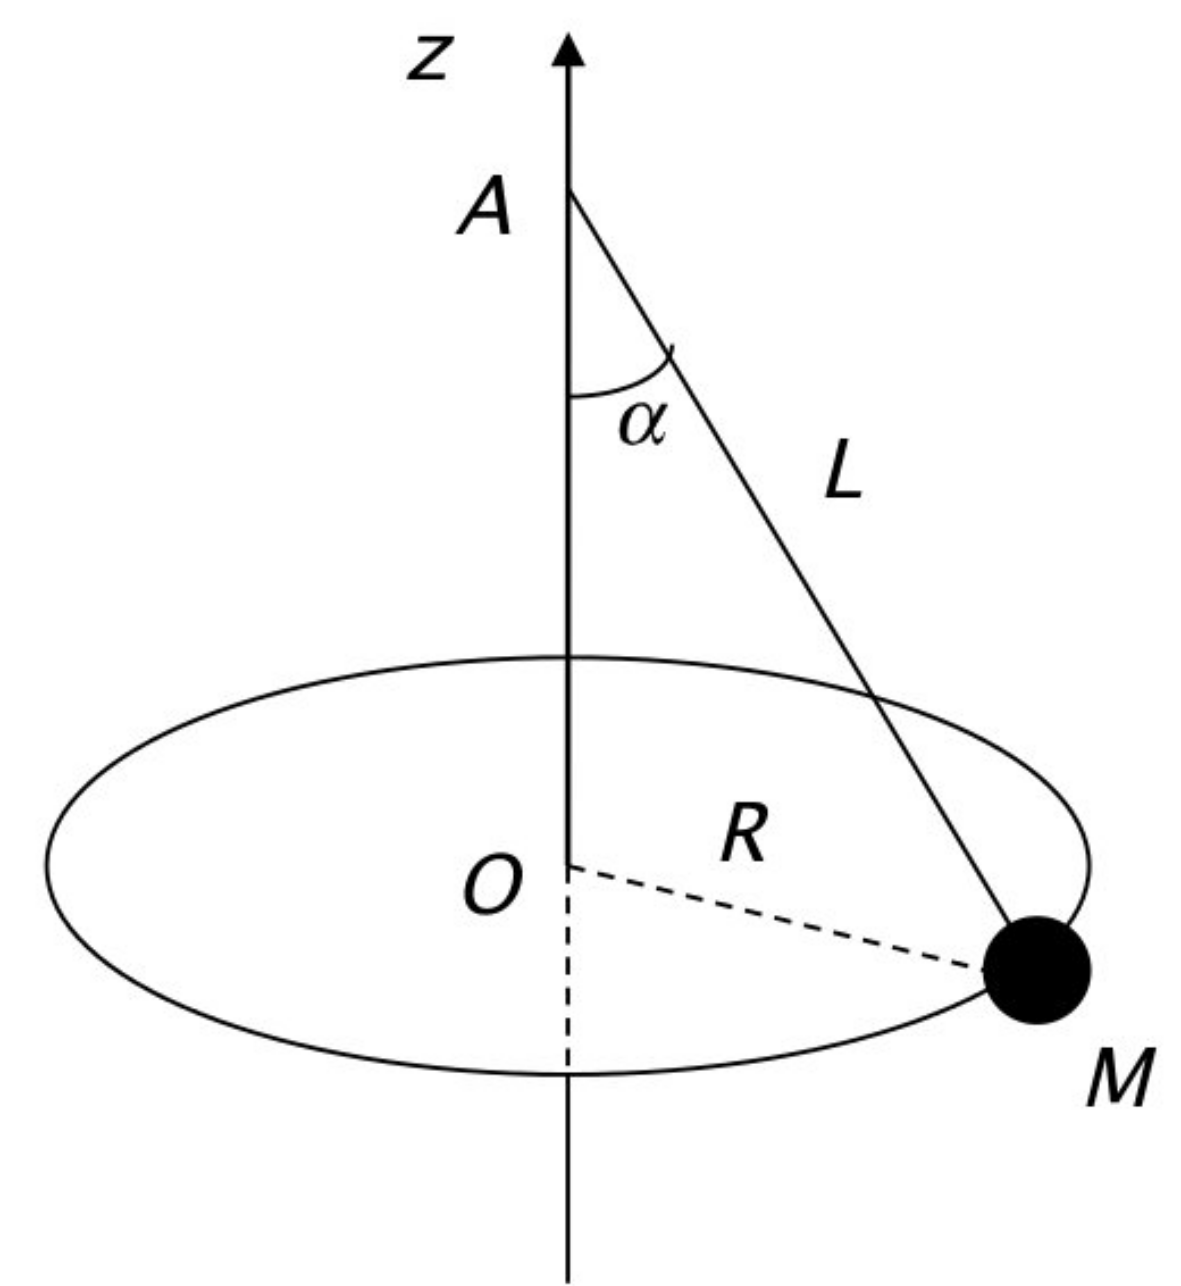
\includegraphics[width=\linewidth]{../../figures/ch17/pendule_conique-plain}
\end{wrapfigure}
Dans un champ uniforme de pesanteur $\gf$ vertical et vers le bas, un point
matériel M de masse $m$ tourne à la vitesse angulaire $\w$ constante autour de
l'axe (O$z$) dirigé vers le haut en décrivant un cercle de centre O et de rayon
$R$. M est suspendu à un fil inextensible de longueur $L$ et de masse
négligeable, fixé en un point A de (O$z$). L'angle $\a$ de (O$z$) avec AM est
constant. \bigbreak
\QR{~
\begin{enumerate}
    \item Quel système de coordonnées utiliser~?
    \item Effectuer un bilan des forces s'appliquant à la masse et les écrire
        dans la base choisie.
    \item Appliquer le PFD puis exprimer $\cos\a$ en fonction de $g$, $L$ et
        $\w$. En déduire que la vitesse angulaire doit forcément être supérieure
        à une vitesse angulaire limite $\w_{\lim}$ pour qu'un tel mouvement
        puisse être possible.
    \item Que dire du cas où $\w$ devient très grande~?
    \item Application numérique~: calculer $\a$ pour $L = \SI{20}{cm}$ et $\w =
        \SI{3}{tours.s^{-1}}$.
\end{enumerate}
}
{
\begin{enumerate}
    \item On utilisera un repère cylindrique pour étudier la rotation.
    \item 
        \begin{itemize}[label=$\diamond$, leftmargin=10pt]
            \litem{Système~:} \{M\} masse $m$
            \litem{Référentiel~:} $\Rc\ind{labo}$ supposé galiléen
            \litem{Repère~:} $(\Or, \ur, \ut, \uz)$ (voir schéma)
        \end{itemize} \smallbreak
        \begin{minipage}{0.65\linewidth}
            \begin{itemize}[label=$\diamond$, leftmargin=10pt]
                \litem{Repérage~:} $R = \cte\Ra\dot{R} = 0$, $\tp = \w =
                    \cte\Ra\dot{\w} = 0$~:
                    \begin{align*}
                        \OM       & = R\ur = L\sin\a\ur\\
                        \vf_{\Mr} & = L\tp\sin\a\ut\\
                                  & = L\w\sin\a\ut\\
                        \af_{\Mr} & = -L\w^2\sin\a\ur
                    \end{align*}
                \litem{BDF~:}
                    \[
                        \begin{array}{ll}
                            \textbf{Poids} & \Pf = m\gf = -mg\uz\\
                            \textbf{Tension} & \Tf = T(-\sin\a\ur + \cos\a\uz)
                        \end{array}
                    \]
            \end{itemize}
        \end{minipage}
        \hfill
        \begin{minipage}{0.30\linewidth}
            \begin{center}
                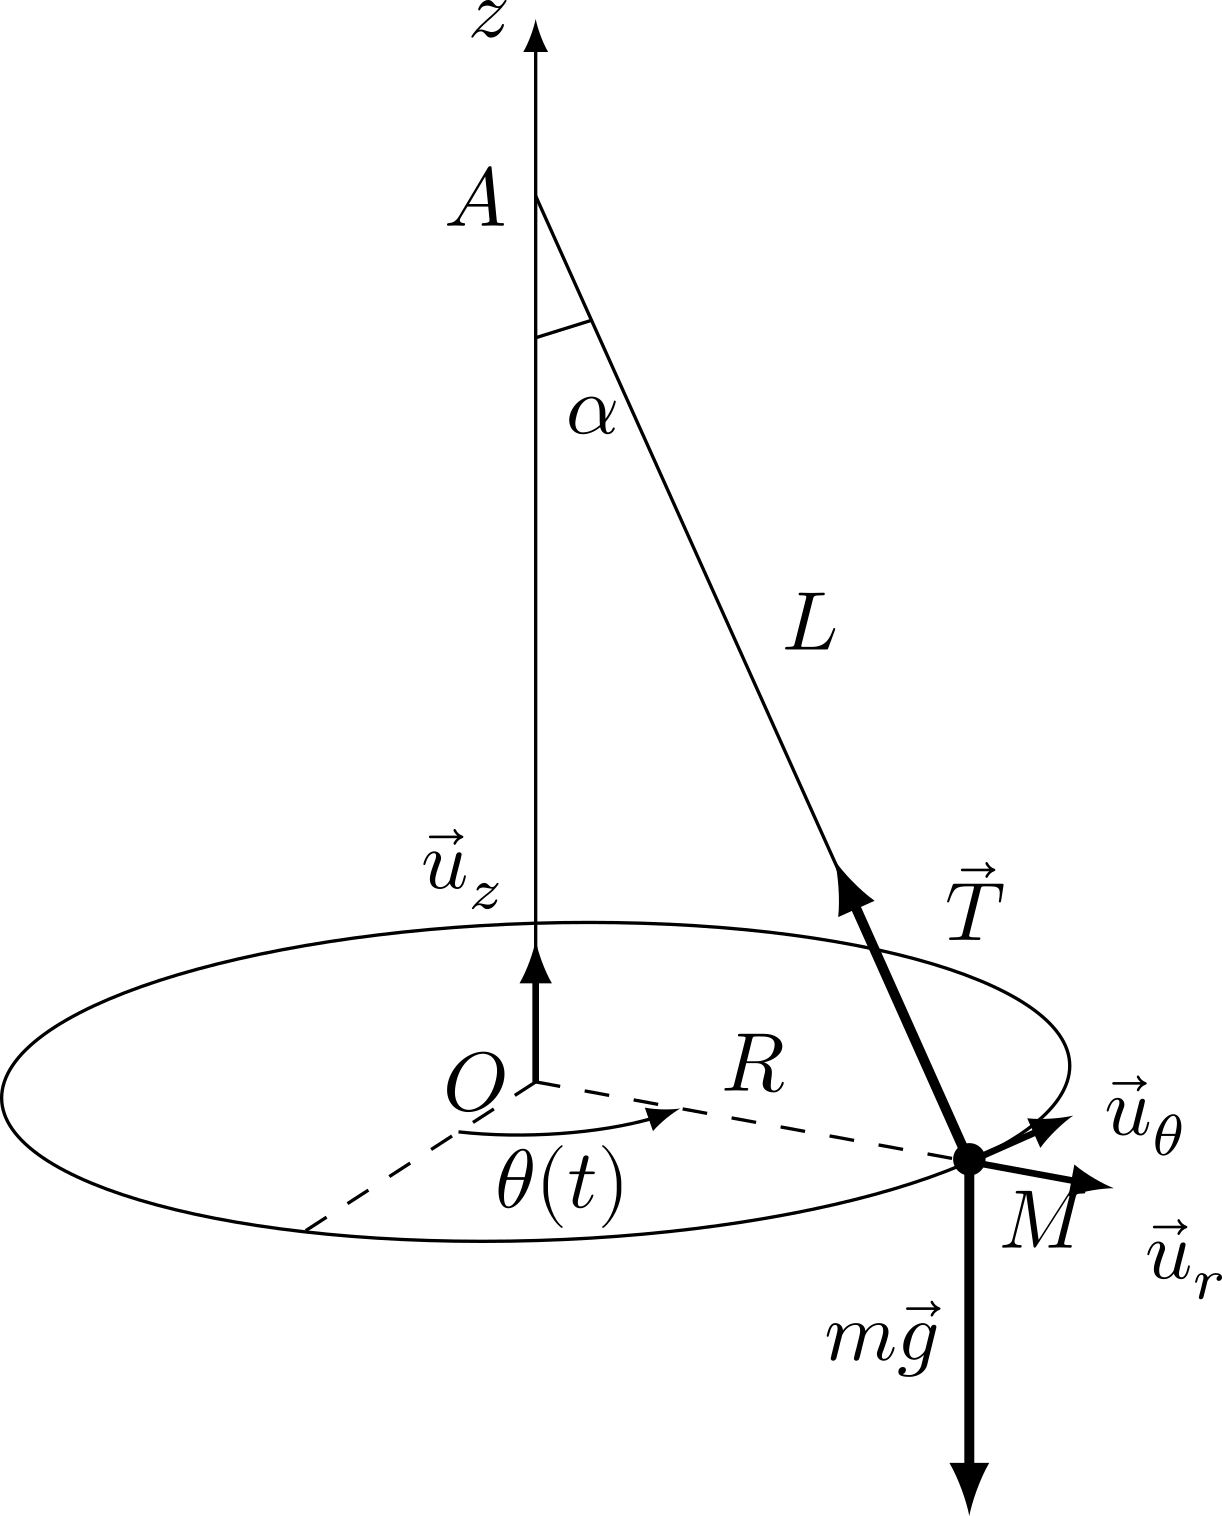
\includegraphics[width=\linewidth]{../../figures/ch17/pendule_corr}
            \end{center}
        \end{minipage}
    \item On applique le PFD~:
        \begin{gather*}
            m\af = \Pf + \Tf
            \Lra
            \left\{
                \begin{aligned}
                    -mL\w^2\cancel{\sin\a} & = -T\cancel{\sin\a}\\
                    0             & = T\cos\a -mg
                \end{aligned}
            \right.
            \Lra
            \left\{
                \begin{aligned}
                    T &= mL\w^2\\
                    T &= \frac{mg}{\cos\a}
                \end{aligned}
            \right.
            \shortintertext{Soit}
            mL\w^2 = \frac{mg}{\cos\a}
            \Lra
            \boxed{\cos\a = \frac{g}{L\w^2}}
        \end{gather*}
        Pour que ce mouvement soit possible, il faut que $\cos\a < 1$, soit
        \begin{gather*}
            \frac{g}{L\w^2} < 1
            \Lra
            \boxed{\w \geq \sqrt{\frac{g}{L}} = \w_{\lim}}
        \end{gather*}
    \item Si $\w \gg \w_{\lim}$, alors $\cos\a \xrightarrow[\w \gg \w_{\lim}]{} 0$
        donc \fbox{$\a\xrightarrow[\w \gg \w_{\lim}]{} \pi/2$}~: le mouvement
        devient simplement circulaire, et se fait dans le plan horizontal
        contenant A.
    \item \leftcenters{On trouve}{\fbox{$\cos\a = \num{0.138} \Lra \a =
        \ang{82}$}}
\end{enumerate}
}

\chapter{Sujet 3\siCorrige{\!\!-- corrig\'e}}
\section{Question de cours}

Retrouver les énergies potentielles de forces classiques (poids, rappel
élastique, force newtonienne en $K/r^2$).

\resetQ
\section{Oscillations d'un anneau sur un cerceau}
\begin{wrapfigure}[5]{R}{0.20\linewidth}
    %\vspace*{-20pt}
    \centering
    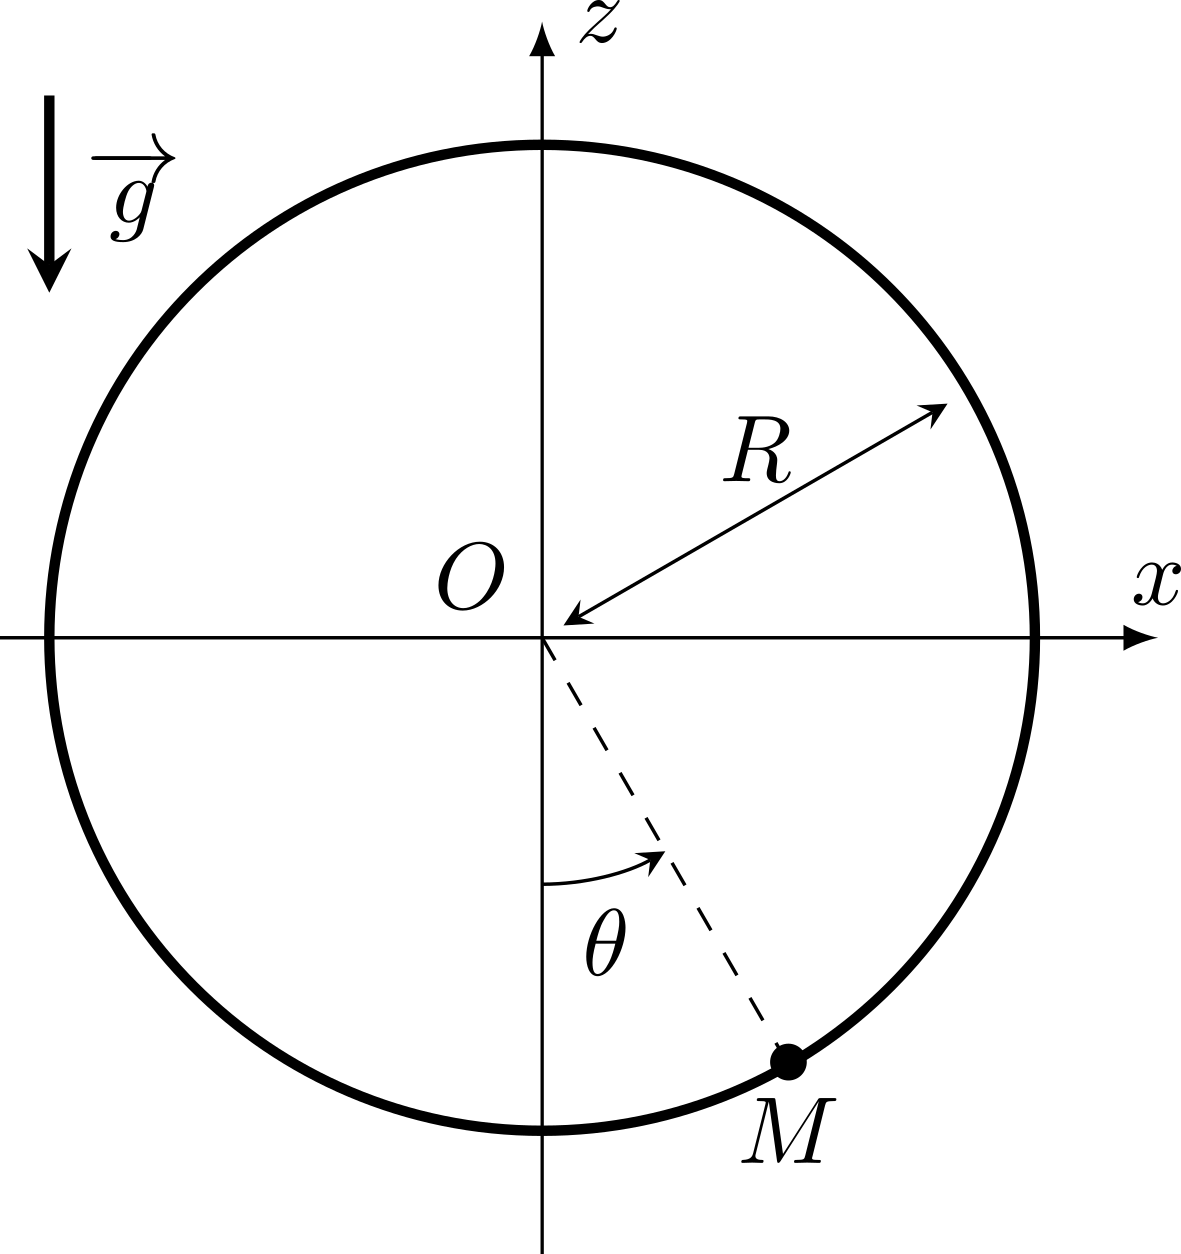
\includegraphics[width=\linewidth]{../../figures/ch17/anneau_cerceau-plain}
\end{wrapfigure}
Un cerceau de centre O et de rayon $R$ est maintenu dans un plan vertical, et un
anneau de masse $m$ assimilé à un point matériel M peut glisser sans frottements
le long de ce cerceau.
\QR{Qu'est-ce que l'hypothèse «~sans frottements~» implique pour la
réaction du cerceau sur l'anneau~?}
{
L'hypothèse «~sans frottements~» signifie que la réaction du cerceau
est uniquement normale~: il n'y a pas de composante tangentielle.
}
\QR{Écrire le PFD appliqué à l'anneau et le projeter dans une base
adaptée.}
{
\begin{itemize}[label=$\diamond$, leftmargin=10pt]
    \litem{Système~:} \{anneau\}
    \litem{Référentiel~:} $\Rc\ind{sol}$ supposé galiléen
    \litem{Repère~:} $(\Or,\ur,\ut)$ avec $\ut$ dans le sens de $\tt$
    \litem{Repérage~:}
        \begin{align*}
            \OM(t) &= R\ur\\
            \vf(t) &= R\tp\ut\\
            \af(t) &= R\tpp\ut - R\tp^2\ur
        \end{align*}
    \litem{BDF~:}
        \[
            \begin{array}{ll}
                \textbf{Poids} & \Pf = mg(\cos\tt\ur -\sin\tt\ut)\\
                \textbf{Réaction} & \Rf = -R_N\ur
            \end{array}
        \]
    \item \leftcenters{\textbf{PFD~:}}{
            $\DS
            m\af = \Pf + \Rf
            \Lra
            \mqty(-mR\tp^2\\mR\tpp) = \mqty(mg\cos\tt-R_N\\-mg\sin\tt)
            $}
            \begin{empheq}[box=\fbox, left=\Lra\empheqlbrace]{align}
                mg\cos\tt + mR\tp^2 & = R_N\notag\\
                \label{eq:pendb}
                mR\tpp + mg\sin\tt & = 0
            \end{empheq}
\end{itemize}
}
\QR{En déduire l'équation différentielle régissant le mouvement.}
{Avec \eqref{eq:pendb}, en la mettant sous forme canonique~:
        \begin{equation}\label{eq:pendc}
            \tpp + \frac{g}{R}\sin\tt = 0
            \Lra
            \boxed{\tpp + \w_0{}^2\sin\tt = 0}
        \end{equation}
        \leftcenters{\hspace{-10pt}avec}{$\DS\boxed{\w_0 = \sqrt{\frac{g}{R}}}$}
}

\enonce{On se place dans l'approximation des petits angles ($\abs{\tt} < \tt_0 =
\ang{20}$). Initialement, l'anneau est situé à la verticale en-dessous de O et
il est lancé vers la droite, avec une vitesse initiale de norme $v_0$.}
\QR{En déduire l'équation horaire du mouvement.}
{On a donc
        \[
            \boxed{\tt(0) = 0}
            \qet
            \vf(0) = v_0\ut = R\tp(0)\ut
            \Lra
            \boxed{\tp(0) = \frac{v_0}{R}}
        \]
        L'équation~\eqref{eq:pendc} se simplifie avec $\sin\tt\approx\tt$, pour
        donner
        \begin{gather*}
            \boxed{\tpp + \w_0{}^2\tt = 0}
            \\\Ra
            \tt(t) = A\cos(\w_0t) + B\sin(\w_0t)
            \shortintertext{Et avec les CI,}
            \tt(0) = 0
            \Lra
            \boxed{A = 0}
            \\
            \tp(0) = \frac{v_0}{R}
            \Lra
            \boxed{B = \frac{v_0}{R\w_0}}
            \\\Ra
            \boxed{
            \tt(t) = \frac{v_0}{R\w_0}\sin(\w_0t)}
        \end{gather*}
}
\QR{À quelle condition sur $v_0$ l'approximation des petits angles
est-elle vérifiée~?}
{La valeur maximale de $\abs{\tt(t)}$ est $v_0/(R\w_0)$, quand le
        sinus vaut $\pm1$. Pour avoir des petits angles, il faut que l'angle
        maximal ne dépasse pas $\tt_0$, soit
        \begin{gather*}
            \frac{v_0}{R\w_0} < \tt_0
            \Lra
            v_0 < \tt_0 R \sqrt{\frac{g}{R}}
            \\\Lra
            \boxed{v_0 < \tt_0 \sqrt{Rg}}
        \end{gather*}
}
\label{LastPage}
\end{document}
